\documentclass[phd,abstract,ackno,listtab,listfig]{wmu/wmu-thesis}
%%-------------------Emacs PostScript "pretty-print" page width (97 columns)-------------------%%
%% This file loads a number of standard packages.  Also included at the end of the file are a number of macros.
%% Math packages-----------------%-------------------------------
\usepackage{amsmath}
%\usepackage{amssymb,mathrsfs}%provides symbols, script text in math mode (conflicts with mathdesign)
%\usepackage{bm}% bold math

%% Text packages-----------------%-------------------------------
\usepackage{textcomp,lmodern}%for special symbols 
%\usepackage[normalem]{ulem}%for strikethroughs
\usepackage[utf8]{inputenc}
\usepackage[T1]{fontenc}%modern font encoding

%% The default font is Latin Modern (replaces Computer Modern).  Following are a number of fonts 
%  with extensive math and symbol support.  To use a particular font, uncomment the associated
%  line.  If mathdesign fonts are used, the amssymb and mathrsfs packages should not be loaded
%  independently.

%% PostScript Fonts--------------%-------------------------------
%\usepackage[osf]{mathpazo}		%URW Palladio (A Palatino/Book Antiqua clone), an old style serif typeface
%\usepackage{mathptmx}				%URW Nimbus Roman (A Times clone), a transitional serif typefaces
%\usepackage[scaled]{helvet}	%URW Nimbus Sans (A Helvetica clone), a sans-serif typeface 
%\renewcommand*\familydefault{\sfdefault} %% Only if the base font of the document is to be sans serif

%% Math Design Fonts-------------%-------------------------------
%\usepackage[urw-garamond]{mathdesign}			%Old style serif typeface
\usepackage[adobe-utopia]{mathdesign}			%Transitional serif typefaces (professional)
%\usepackage[bitstream-charter]{mathdesign}	%Glyphic serif typeface optimized for low-resolution printing

%% Formatting packages-----------%-------------------------------
\usepackage{fancyvrb}%allows verbatim in footnotes
\usepackage{indentfirst}%indents first paragraph of each section

\usepackage{hyperref}
\hypersetup{
	pdfstartpage=1,                %Opening page number (absolute)
	pdfstartview=FitV,             %Fits the horiz. width in the window (FitV for vertical)
	%pdfstartview={XYZ null null 1},%view page at 100%
	bookmarksopen=true,            %Displays Bookmarks in the Navigation Panel
	bookmarksopenlevel=0,          %\maxdimen all levels, 0 chapters, 1 sections
	bookmarksnumbered=true,        %Numbers bookmarks with section numbers
	final=true,                    %keeps hyperref features in draft mode
	colorlinks=true,               %colors the links instead of using boxes
	urlcolor=blue,                 %makes URL hyperlinks blue (instead of pink)
	linkcolor=black,               %makes internal links black (instead of red)
	citecolor=black,               %makes citation links black (instead of green)
}

\usepackage{fmtcount,datetime} %provides commands for displaying times and dates
\usepackage{setspace} %required for double spacing and used to control vertical spacing 
\usepackage[numbers,sort&compress]{natbib}
\usepackage{fancyhdr} %required for non-standard (fancy) headers

%% The following two lines may be required for proper formatting of the Table of Figures
%\usepackage{tocloft}
%\setlength{\cftfignumwidth}{3em}%increases spacing after figure numbers in Table of Figures

\usepackage{color}

\InputIfFileExists{src/autotext}{}{}

\renewcommand{\thefootnote}{\fnsymbol{footnote}} %sets footnote marks to symbols

\providecommand{\Chapter}[1]{\chapter[\texorpdfstring{\MakeUppercase{#1}}{#1}]{#1}}
\begin{document}
%% Personal information----------%-------------------------------
\renewcommand{\authname}{Author Name}
\renewcommand{\thesistitle}{\MakeUppercase{Dissertation Title}}
\renewcommand{\gradyear}{2011}
\renewcommand{\gradmonth}{6}
\renewcommand{\departmentname}{Department Name}
\renewcommand{\adviname}{Advisor Name,Ph.D.}
\frontmatter
\mainmatter
\providecommand{\Chapter}[1]{\chapter[\texorpdfstring{\MakeUppercase{#1}}{#1}]{#1}}
%% Main text---------------------%-------------------------------
\Chapter{Introduction}
The quick brown fox jumps over a lazy dog~\cite{Lighthall_2010}.
\begin{figure}[!ht]
\centering
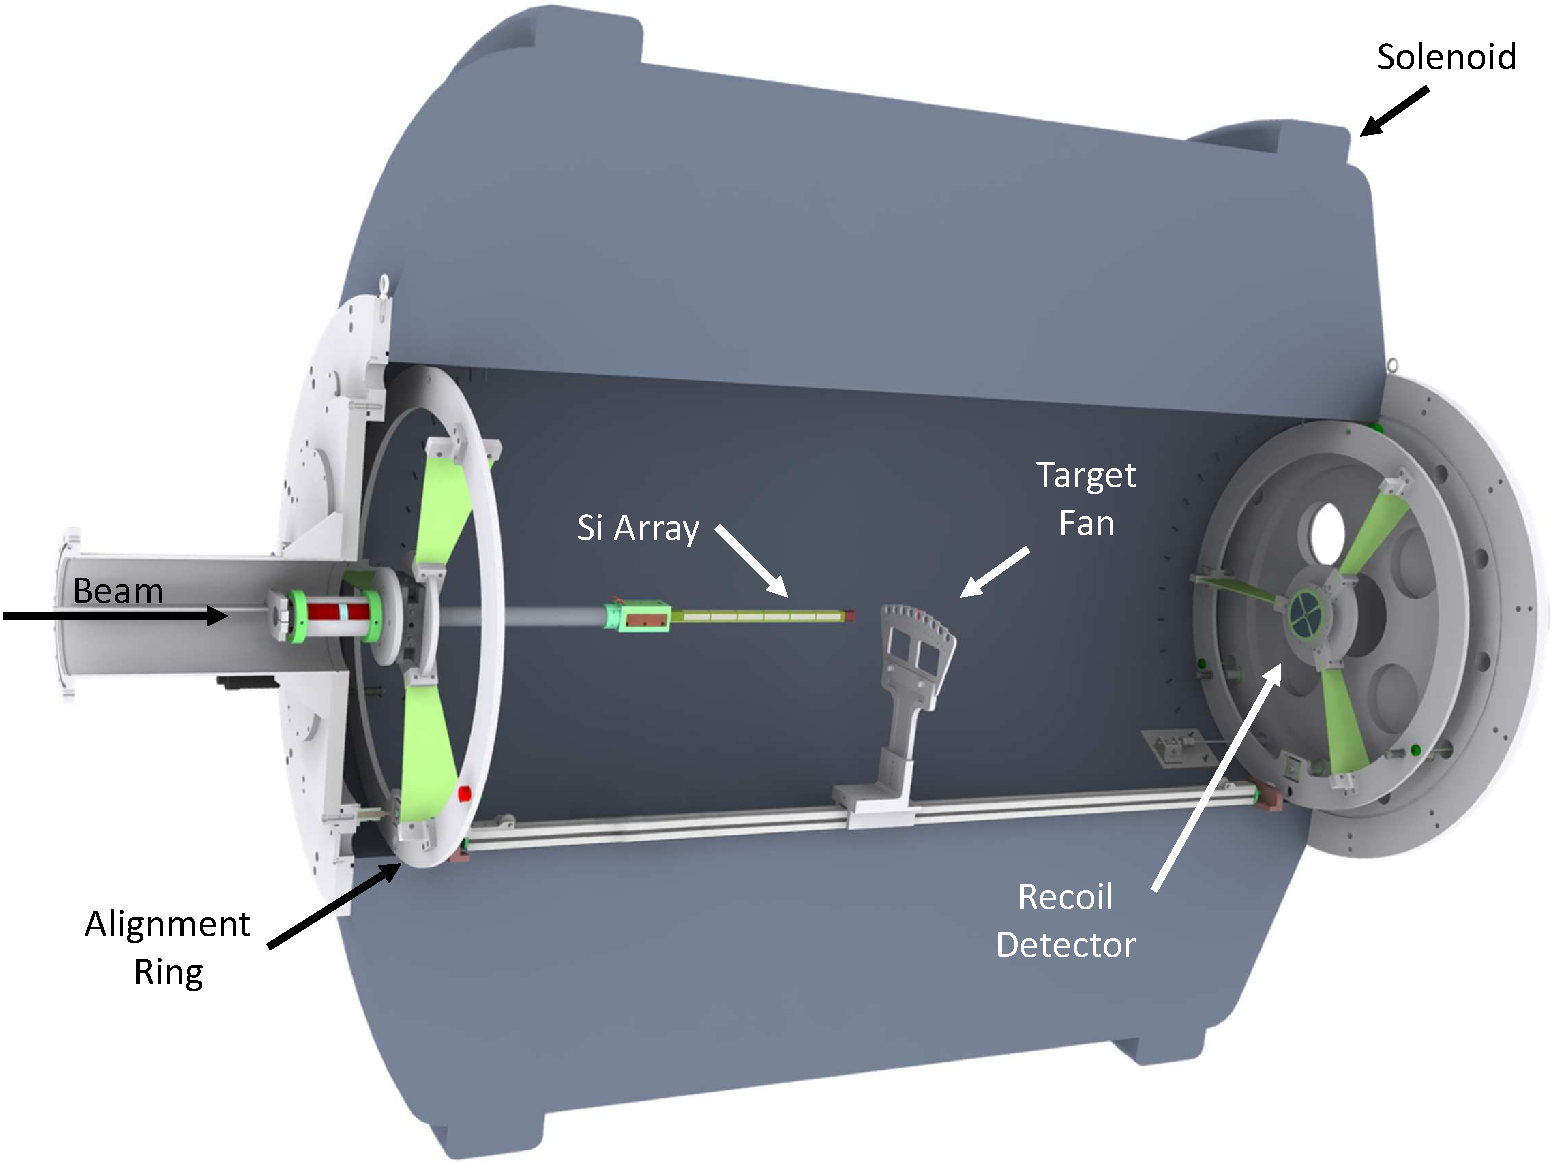
\includegraphics[width=\linewidth,height=0.5\textheight,keepaspectratio]{18pt_rot3}
\caption[Cutaway schematic view of HELIOS in the ``($d$,$p$)'' configuration]{Cutaway schematic view of HELIOS in the ``($d$,$p$)'' configuration.  The accelerated beam enters from left.  Shown are the light-ion silicon detector array suspended on the upstream alignment ring, rotating target fan, and heavy-recoil detector.  Mechanical design by S.~Heimsath.  3D rendering by B.~J.\ DiGiovine.  This figure also appears in Ref.~\cite{Lighthall_2010}.}
\label{schematic}
\end{figure}

%% References--------------------%-------------------------------
\renewcommand{\bibname}{References}%Set the name of the bibliography here
\cleardoublepage
\phantomsection 
\begin{thebibliography}{999}
\bibitem{Lighthall_2010}
J.~C. Lighthall \emph{et~al.}, Nucl.\ Instr.\ and Meth.\ A\textbf{ 622} 97--106 (2010).
\end{thebibliography}
\addcontentsline{toc}{chapter}{\texorpdfstring{\uppercase{\bibname}}{\bibname}}
\twoappendix
\Chapter{Title}
The quick brown fox jumps over a lazy dog.
\end{document}
